\section{Methodology}
\label{sec:method}

In this section, we present the computational strategy used for computing the active subspace in the case of
H$_2$/O$_2$ reaction kinetics with uncertain pre-exponent of individual reaction rates provided in
Table~\ref{tab:kinetics}. Specifically, we employ two strategies: One that involves computation of model
gradients in order to construct the matrix (grad-based), $\mat{C}$ in~\eqref{eq:chat}, and the other that involves a local 
linear approximation of the model output to circumvent the computational cost associated with gradient
computation (grad-free). The grad-based approach is based on Algorithm 1.1, and the grad-free approach is
based on Algorithm 1.2 in~\cite{Constantine:2015}. However, in this work, we have implemented the
two strategies in an iterative manner and have demonstrated potential for additional savings in both cases.
Additionally, for the present application, our findings based on the two strategies are observed to be consistent.
Since, the grad-free approach is relatively more efficient, this observation encourages its use for high-dimensional
applications as discussed later in Section~\ref{sec:app}. Note however, that the model output is required to be
differentiable throughout the input domain in both cases.

\subsection{Grad-based approach}
\label{sub:grad}

As discussed earlier, in the grad-based approach, the elements of $\mat{C}$ are estimated using model gradients.
 In situations where the gradient is not available analytically, one could consider using
finite difference and other relatively more efficient techniques such as automatic differentiation~\cite{Kiparissides:2009} 
and adjoint-based gradient computation~\cite{Jameson:1988,Gunzburger:2003,Borzi:2011,Alexanderian:2017}.
Model evaluations at neighbouring points are required if finite difference is used. Hence, for 
$N$ samples in a $d$-dimensional parameter space, $N(d+1)$ model evaluations are needed. 

We begin by evaluating the gradient of the model output, $\nabla_{\bm{\xi}}f$, at an initial set of $n_1$ samples. 
For this purpose, $\bm{\xi}_i$'s are projected to the physical space as $\bm{\theta}_i$'s. Using the gradient
evaluations, the matrix, $\mat{C}$ is computed. Eigenvalue decomposition of $\mat{C}$ yields an initial
estimate of the dominant eigenspace, $\bm{W}_1$ and corresponding set of eigenvalues, $\bm{\Lambda}_1$.
At each subsequent iteration, model evaluations are generated at a new set of $n_s$ samples. The new set
of gradient evaluations are augmented with the available set to re-construct $\mat{C}$ followed by its eigenvalue
decomposition. The relative
change in the norm of the difference in individual components of the dominant eigenvectors between subsequent 
iterations is evaluated. The process is terminated and the resulting eigenspace is considered to be converged once the
relative change, $\delta w_{1,j}^{(r)}$, is smaller a given tolerance, $\tau$. A regression fit to
 $G(\bm{w}_1^\top\bm{\xi})$ is used as a surrogate to characterize and quantify the uncertainty in the model
 output. Moreover, the components of the dominant eigenvectors are used to compute the activity scores which
 provide an insight into the relative importance of the uncertain parameters. The sequence of steps for the grad-based
 approach are provided in Algorithm~\ref{alg:grad}.

%% Grad-based algorithm

\bigskip
\begin{breakablealgorithm}
\renewcommand{\algorithmicrequire}{\textbf{Input:}}
\renewcommand{\algorithmicensure}{\textbf{Output:}}
  \caption{An iterative gradient-based approach for discovering the active subspace}
  \begin{algorithmic}[1]
\Require $\theta_l$, $\theta_u$, $\tau$. 
\Ensure $\Lambda$, $W$, $\eta$. 
    \Procedure{Gradient-based}{}
	\State Draw $n_1$ random samples, $\{\bm{\xi}_k\}_{k=1}^{n_1}$ $\in$ [-1,1]
         according to $\bm{f(\xi)}$.
	\State Project to the physical space:
        $\{\bm{\theta}_k\}_{k=1}^{n_1}=\theta_l+0.5(\theta_u-\theta_l)\{\bm{\xi}_k\}_{k=1}^{n_1}$
	\State $N_\text{total}$ = $n_1$ 
	\State Compute $\bm{g}^k = \nabla_{\bm{\theta}}G(\bm\theta_k)$, 
             $k=1, \ldots, N_\text{total}$.  
	\Statex\hspace{5mm} Using Finite Difference:
	\Statex\hspace{5mm} i. Assign a small increment, $d\xi$.
	\Statex\hspace{5mm} ii. Augment the set of samples with neighboring points.
	\be \{\bm{\Xi}_k\}_{k=1}^{n_1(N_p+1)}:~\{\bm{\xi}_k\}_{k=1}^{n_1} \cup
        \{\xi_{k,j}+d\xi\}_{j=1}^{N_p} \nonumber
	\ee
	\Statex\hspace{5mm} iii. Project to the physical space:
        $\{\bm{\theta}_k\}_{k=1}^{n_1(N_p+1)}=\theta_l+0.5(\theta_u-\theta_l)\{\bm{\Xi}_k\}_{k=1}^{n_1(N_p+1)}$
	\Statex\hspace{5mm} iv. Using the augmented set, $\{\bm{\theta}_k\}_{k=1}^{n_1(N_p+1)}$
        to compute $\bm{g}^k$. 
	\State Compute the matrix, $\mathcal{C}$ = 
        $\frac{1}{N_\text{total}}\sum\limits_{k=1}^{N_\text{total}}[\bm{g}^k][\bm{g}^k]^\top$
	\State Eigenvalue decomposition, $\mathcal{C}$ = $W^{(0)}\Lambda^{(0)} W^{(0)\top}$
	\State Partition the Eigenpairs: $\Lambda^{(0)}~=~ 
        \begin{bmatrix} \Lambda_1^{(0)} & \\ & \Lambda_2^{(0)} \end{bmatrix}$, 
        $W^{(0)}~=~\begin{bmatrix} w_1^{(0)} & w_2^{(0)} \end{bmatrix}$, 
        $\Lambda_1^{(0)}\in \mathbb{R}^{N_p\times\mathcal{S}}$
	\State Set $r$ = 0
	\Loop
		\State Set $r$ = $r$ + 1
		\State Draw $n_r$ = $\lceil \beta n_1 \rceil$ new random samples 
                $\{\bm{\xi}_k\}$ $\in$ [-1,1], $k = n_{r-1}+1,\ldots,n_{r-1}+n_r$.
		\State Project $\bm{\xi}_k$~$\rightarrow$~$\bm{\theta}_k$.
		\State $N_\text{total}$ = $N_\text{total}$ + $n_r$ 
		\State Compute $\bm{g}^k = \nabla_{\bm{\theta}}G(\bm\theta_k)$, 
             	$k=n_{r-1}+1, \ldots, n_{r-1}+n_r$.  
		\State Compute $\mathcal{C}$ = 
        	$\frac{1}{N_\text{total}}\sum\limits_{k=1}^{N_\text{total}}[\bm{g}^k][\bm{g}^k]^\top$
		\State Eigenvalue decomposition, $\mathcal{C}$ = $W^{(r)}\Lambda^{(r)} W^{(r)\top}$
		\State Compute $\delta w_{1,j}^{(r)}$ = 
                       \scalebox{1.25}{$\frac{\|w_{1,j}^{r} - 
                       w_{1,j}^{r-1}\|}{\|w_{1,j}^{r-1}\|}$}, 
                       $j = 1,\ldots,\mathcal{S}$.
		\If {$\max\left(\delta w_{1,j}^{(r)}\right)<\tau$}
			\State break
		\EndIf
	\EndLoop
	\State Compute $\eta_i(N_\text{total}) = \sum\limits_{j=1}^{\mathcal{S}} \Lambda_{1,j}w_{1,j}^2$,
	$i=1,\ldots,d$.
	
    \EndProcedure
  \end{algorithmic}
  \label{alg:grad}
\end{breakablealgorithm}
\bigskip

In order to motivate the iterative strategy used in this work, we implement Algorithm~\ref{alg:grad} to the
19-dimensional H$_2$/O$_2$ reaction kinetics problem with uncertain $A_i$'s. For the purpose of
verification, $\mat{C}$ is initially constructed using a large set of samples ($N$~=~1000) in the input
domain and the corresponding active subspace is computed. In Figure~\ref{fig:eig_comp}(a), we illustrate
the comparison of the resulting eigenvalue spectrum ($\lambda_1 - \lambda_{19}$) with the same using a much 
smaller set of samples, $n$~=~$\{20,40,80,120\}$. Additionally, in Figure~\ref{fig:eig_comp}(b), we compare
relative L-2 norm of the difference between the first five eigenvectors of $\mat{C}$.
%
\begin{figure}[htbp]
 \begin{center}
  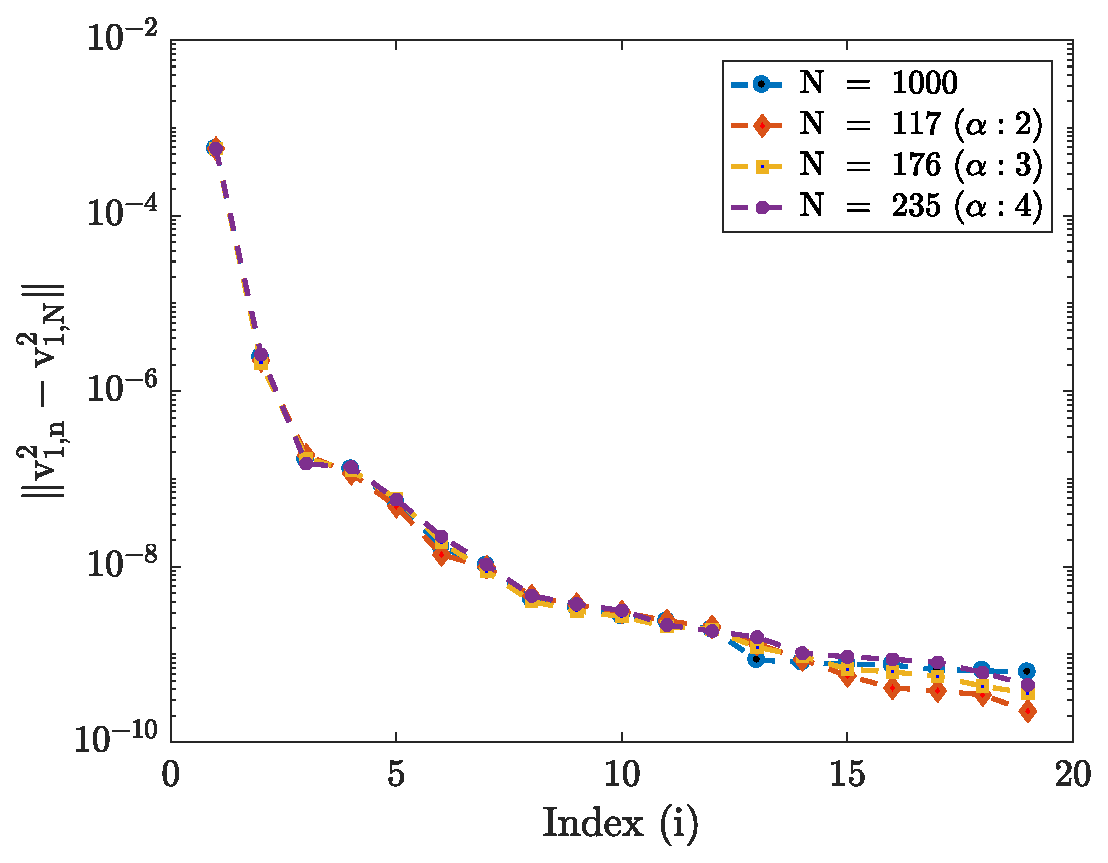
\includegraphics[width=0.45\textwidth]{./Figures/eig_comp}
   \includegraphics[width=0.48\textwidth]{./Figures/err_eigv_1_5}
\caption{Left: A comparison of the eigenvalue spectrum using $n$ = $\{20,40,80,120\}$ samples with that
obtained using a much larger sample size, $N$~=~1000. Right: Relative L-2 norm of the difference between
individual components of the first five eigenvectors of $\mat{C}$, constructed using $N$~=~1000 samples,
and using a smaller sample size, $n$ ranging from 20 to 240.} 
\label{fig:eig_comp}
\end{center}
\end{figure}
%
Interestingly, we observe that the dominant eigenvalues~($\lambda_1 - \lambda_4$) are approximated 
reasonably well with just 20 samples. As expected, the accuracy of higher-order eigenvalues is observed
to improve with the sample size. Similarly, the relative error associated with the dominant eigenvectors
($i$ = 1,2) is found to range from $\mathcal{O}(10^{-2} - 10^{-1})$ and is relatively much smaller than 
the higher-order eigenvalues. In this case, since $\left(\frac{\lambda_1}{\lambda_2}\right)\gg 1$, we have
a 1-dimensional active subspace. Hence, the first eigenvector sufficiently captures the uncertainty in
the  model output. Therefore, a sample size of 20 is adequate for computing the active subspace in this
case. The iterative strategy therefore offers a significant potential for computational advantage. 
However, estimating the gradient of the model output imposes a significant computational burden.
Hence, we explore the applicability of a so-called gradient-free approach as mentioned earlier, in the
following section.  

\subsection{Grad-free approach}
\label{sub:gradfree}

\bigskip
\begin{breakablealgorithm}
\renewcommand{\algorithmicrequire}{\textbf{Input:}}
\renewcommand{\algorithmicensure}{\textbf{Output:}}
  \caption{An iterative gradient-free approach for discovering the active subspace}
  \begin{algorithmic}[1]
\Require $\theta_l$, $\theta_u$, $\tau$. 
\Ensure $\Lambda$, $W$, $\eta$. 
    \Procedure{Gradient-free}{}
	\State Assign $\alpha$ = 3, $q$ = $N_p$+1
	\State Set $M$ = $\lfloor\alpha q\log(N_p)\rfloor$
	\State Draw $n_1$ random samples, $\{\bm{\xi}_k\}_{k=1}^{n_1}$ $\in$ [-1,1]
         according to $\bm{f(\xi)}$.
	\State Project to the physical space:
        $\{\bm{\theta}_k\}_{k=1}^{n_1}=\theta_l+0.5(\theta_u-\theta_l)\{\bm{\xi}_k\}_{k=1}^{n_1}$
	\State $N_\text{total}$ = $n_1$ 
	\State Compute $G(\bm\theta_k)$, $k=1, \ldots, N_\text{total}$.
	\State Draw $M$ random samples, $\{\bm{\nu}_k\}_{k=1}^{M}$ $\in$ [-1,1]
         according to $\bm{f(\xi)}$.
	\State Construct the matrix, $\mathcal{C}$.
	\State Eigenvalue decomposition, $\mathcal{C}$ = $W^{(0)}\Lambda^{(0)} W^{(0)\top}$
	\State Partition the Eigenpairs: $\Lambda^{(0)}~=~ 
        \begin{bmatrix} \Lambda_1^{(0)} & \\ & \Lambda_2^{(0)} \end{bmatrix}$, 
        $W^{(0)}~=~\begin{bmatrix} w_1^{(0)} & w_2^{(0)} \end{bmatrix}$, 
        $\Lambda_1^{(0)}\in \mathbb{R}^{d\times\mathcal{S}}$
	\State Set $r$ = 0
	\Loop
		\State Set $r$ = $r$ + 1
		\State Draw $n_r$ = $\lceil \beta n_1 \rceil$ new random samples 
                $\{\bm{\xi}_k\}$ $\in$ [-1,1], $k = n_{r-1}+1,\ldots,n_{r-1}+n_r$.
		\State Project $\bm{\xi}_k$~$\rightarrow$~$\bm{\theta}_k$.
		\State $N_\text{total}$ = $N_\text{total}$ + $n_r$ 
		\State Compute $G(\bm\theta_k)$, $k=n_{r-1}+1, \ldots, n_{r-1}+n_r$.  
		\State Construct the matrix, $\mathcal{C}$.
		\State Eigenvalue decomposition, $\mathcal{C}$ = $W^{(r)}\Lambda^{(r)} W^{(r)\top}$
		\State Compute $\delta w_{1,j}^{(r)}$ = 
                       \scalebox{1.25}{$\frac{\|w_{1,j}^{r} - 
                       w_{1,j}^{r-1}\|}{\|w_{1,j}^{r-1}\|}$}, 
                       $j = 1,\ldots,\mathcal{S}$.
		\If {$\max\left(\delta w_{1,j}^{(r)}\right)<\tau$}
			\State break
		\EndIf
	\EndLoop
	\State Compute $\eta_i(N_\text{total}) = \sum\limits_{j=1}^{\mathcal{S}} \Lambda_{1,j}w_{1,j}^2$,
	$i=1,\ldots,d$.
    \EndProcedure
  \end{algorithmic}
  \label{alg:free}
\end{breakablealgorithm}
\bigskip

%\bigskip
%\begin{breakablealgorithm}
%\renewcommand{\algorithmicrequire}{\textbf{Input:}}
%\renewcommand{\algorithmicensure}{\textbf{Output:}}
%  \caption{Algorithm for constructing the matrix, $\mathcal{C}$}
%  \begin{algorithmic}[1]
%\Require $N_\text{total}$, $M$, $\{G(\bm\theta_k)\}_{k=1}^{N_\text{total}}$, 
%$\{\bm{\xi}_k\}_{k=1}^{N_\text{total}}$,
%         $\{\bm{\nu}_k\}_{k=1}^{M}$. 
%\Ensure $\mathcal{C}$. 
%    \Procedure{Matrix $\mathcal{C}$}{}
%	\State Set $p$ = $N_\text{total}$ - 1
%	\State Initialize $\mathcal{D}$ = $[0,\ldots,0]^\top$, $\mathcal{D}\in
%                            \mathbb{R}^{N_\text{total}\times 1}$
%	\For{$i$ = 1 to $M$}
%	\For {$j$ = 1 to $N_\text{total}$}
%	\State $\mathcal{D}(j)$ = 0
%	\For {$k$ = 1 to $d$}
%	\Statex\hspace{20mm} $\mathcal{D}(j) = \mathcal{D}(j) + \|\nu(i,k) - \xi(j,k)\|$
%	\EndFor
%	\EndFor
%	\State $[z,index(i,:)]$ = sort($\mathcal{D}$)
%	\For {$j$ = 1 to $p$}
%	\State $ip = (i-1)p + j$
%	\State $points(ip,:) = \xi(index(i,j),:)$
%	\EndFor
%	\EndFor
%	\For{$np$ = 1 to $M$}
%	\State $A$ = [1 $points((np-1)p+1,:)$]
%	\For{$i$ = $(np-1)p+2$ to ($np\ast p$)}
%	\State $A=[A; 1~points(i,:)]$
%	\EndFor
%	\State $B = G(index(np,1))$
%	\For{$i$ = 2 to $p$}
%	\State $B = [B;~G(index(np,i))]$
%	\EndFor
%	\State $z = A\setminus B$
%	\If {$np$ == 1}
%	\State $\mathcal{B} = z(2:N_p+1)$	
%	\Else 
%	\State $\mathcal{B} = [\mathcal{B}~z(2:N_p+1)]$
%	\EndIf
%	\EndFor
%	\State $\mathcal{C}$ = 0
%	\For {$i$ = 1 to $M$}
%	\State $z$ = $\mathcal{B}(:,i)$
%	\State $\mathcal{C}=\mathcal{C}+zz^\top$
%	\EndFor
%	\State $\mathcal{C}=\mathcal{C}/M$
%    \EndProcedure
%  \end{algorithmic}
%  \label{alg:C}
%\end{breakablealgorithm}
%\bigskip
